%%%%%%%%%%%%%%%%%%%%%%%%%%%%%%%%%%%%%%%%%
% Appendix
% 
% $Date$
% $Rev$:
% $Author$


\appendix

\chapter*{Appendix}
\addcontentsline{toc}{chapter}{Appendix}
\addtocontents{toc}{\protect\setcounter{tocdepth}{-1}}

\chapter{Wrapper scripts}

The \dir{bin/} directory of the binary release contains some \file{.sh}  and %
\file{.bat} scripts to invoke tools included in the \mainJar{}. %
The following sections give a short description of their functionality and %
list their usage outputs as listed when called without command-line parameters. %

% generated by the script gen-bin-usage-tex.sh with manual adjustments

\section{Script \file{convertLoggingTimestamp.sh|bat}}

\paragraph*{Usage}\

\setTextListing
\lstinputlisting[caption=]{Appendix-usage-convertLoggingTimestamp.sh.inc}

\paragraph*{Example}

\setBashListing
\begin{lstlisting}
#\lstshellprompt{}# 
\end{lstlisting}


\chapter{\KiekerMonitoringPart{} Configuration File}\label{sec:appdx:monitoringproperties}

This is the file \file{\monitoringPropertiesFile} from the binary release and 
constitutes \KiekerMonitoringPart{}'s default configuration.

\

\setXMLListing
\lstinputlisting[caption=\monitoringPropertiesFile]{../../META-INF/kieker.monitoring.properties}

\chapter{Additional Source Code Listings}
\section{MyNamedPipeManager and MyPipe}\label{appendix:pipeListings}
      \setJavaCodeListing
      \lstinputlisting[caption=MyNamedPipeManager.java]{\customComponentsBookstoreApplicationDir/src/bookstoreApplication/MyNamedPipeManager.java}
\newpage
      \setJavaCodeListing
      \lstinputlisting[caption=MyPipe.java]{\customComponentsBookstoreApplicationDir/src/bookstoreApplication/MyPipe.java}

\chapter{Example Console Outputs}

\section{Quick Start Example (Chapter~\ref{chap:example})}\label{sec:appendix:manualInstrumentation:output}
% \subsubsection{Monitoring}
% 		The following listing shows the produced log during a run of the Bookstore Application with the manual monitoring probes.
\setTextListing
\begin{lstlisting}[caption=Execution of the manually instrumented Bookstore application (Section~\ref{sec:example:monitoring})]
Apr 28, 2011 5:15:25 PM kieker.monitoring.core.configuration.Configuration createSingletonConfiguration
INFO: Loading properties from properties file in classpath: 'META-INF/kieker.monitoring.properties'
Apr 28, 2011 5:15:25 PM kieker.monitoring.core.configuration.Configuration loadConfigurationFromResource
WARNING: File 'META-INF/kieker.monitoring.properties' not found in classpath
Apr 28, 2011 5:15:25 PM kieker.monitoring.core.controller.MonitoringController createInstance
INFO: Current State of kieker.monitoring (1.3-20110427) Status: 'enabled'
	Name: 'KIEKER-SINGLETON'; Hostname: 'Kaapstad'; experimentID: '1'
WriterController:
	Number of Inserts: '0'
	Automatic assignment of logging timestamps: 'true'
Writer: 'kieker.monitoring.writer.filesystem.AsyncFsWriter'
	Configuration:
		kieker.monitoring.writer.filesystem.AsyncFsWriter.QueueFullBehavior='0'
		kieker.monitoring.writer.filesystem.AsyncFsWriter.QueueSize='10000'
		kieker.monitoring.writer.filesystem.AsyncFsWriter.customStoragePath=''
		kieker.monitoring.writer.filesystem.AsyncFsWriter.storeInJavaIoTmpdir='true'
	Writer Threads (1): 
		Finished: 'false'; Writing to Directory: '/tmp/kieker-20110428-151525684-UTC-Kaapstad-KIEKER-SINGLETON'
Sampling Controller: Periodic Sensor available: Current Poolsize: '0'; Scheduled Tasks: '0'
Bookstore.main: Starting request 0
Bookstore.main: Starting request 1
Apr 28, 2011 5:15:25 PM kieker.monitoring.writer.filesystem.MappingFileWriter writeMapping
INFO: Registered monitoring record type with id '1':kieker.common.record.OperationExecutionRecord
Bookstore.main: Starting request 2
Bookstore.main: Starting request 3
Bookstore.main: Starting request 4
\end{lstlisting}

\newpage
% \subsubsection{Analysis}
% 		The second listing is the log during the analysis of the produced data. It can be seen that some of the calls are accepted and some others refused.
\setTextListing
\begin{lstlisting}[caption=Execution of the example analysis (Section~\ref{sec:example:analysis})]
19.08.2010 13:19:55 kieker.analysis.AnalysisController registerPlugin
INFO: Registered plugin bookstoreApplication.Consumer@6ac2a132
19.08.2010 13:19:55 kieker.analysis.AnalysisController registerPlugin
INFO: Plugin bookstoreApplication.Consumer@6ac2a132 also registered as record consumer
19.08.2010 13:19:55 kieker.analysis.reader.filesystem.FSDirectoryReader processInputFile
INFO: < Loading C:\Temp\tpmon-20100814-103954167-UTC\tpmon-20100814-103954184-UTC-Thread-2.dat
19.08.2010 13:19:55 kieker.common.record.MonitoringRecordTypeRegistry registerRecordTypeIdMapping
INFO: Registered record type mapping 1/kieker.common.record.OperationExecutionRecord
maximal response time exceeded by 11382559 ns: bookstoreApplication.Catalog.getBook()
maximal response time exceeded by 11251720 ns: bookstoreApplication.Catalog.getBook()
maximal response time exceeded by 80320 ns: bookstoreApplication.Catalog.getBook()
maximal response time exceeded by 27400 ns: bookstoreApplication.Catalog.getBook()
maximal response time exceeded by 81760 ns: bookstoreApplication.Catalog.getBook()
maximal response time exceeded by 24240 ns: bookstoreApplication.Catalog.getBook()
maximal response time exceeded by 82480 ns: bookstoreApplication.Catalog.getBook()
response time accepted: bookstoreApplication.Catalog.getBook()
response time accepted: bookstoreApplication.Catalog.getBook()
response time accepted: bookstoreApplication.Catalog.getBook()
14.08.2010 12:41:02 kieker.analysis.reader.filesystem.FSReader$\$$FSReaderCons execute
INFO: All reader threads provided FS_READER_TERMINATION_MARKER
\end{lstlisting}
\newpage	
\section{Trace Monitoring, Analysis \& Visualization (Chapter \ref{chap:aspectJ})}
\setTextListing
\begin{lstlisting}[caption=Execution of the Bookstore with AspectJ trace instrumentation (Section~\ref{sec:traceAnalysis:instr:AspectJ})]
Bookstore.main: Starting request 0
Apr 28, 2011 4:28:29 PM kieker.monitoring.core.configuration.Configuration createSingletonConfiguration
INFO: Loading properties from properties file in classpath: 'META-INF/kieker.monitoring.properties'
Apr 28, 2011 4:28:29 PM kieker.monitoring.core.controller.MonitoringController createInstance
INFO: Current State of kieker.monitoring (1.3-20110427) Status: 'enabled'
	Name: 'KIEKER'; Hostname: 'Kaapstad'; experimentID: '1'
WriterController:
	Number of Inserts: '0'
	Automatic assignment of logging timestamps: 'true'
Writer: 'kieker.monitoring.writer.filesystem.AsyncFsWriter'
	Configuration:
		kieker.monitoring.writer.filesystem.AsyncFsWriter.QueueFullBehavior='0'
		kieker.monitoring.writer.filesystem.AsyncFsWriter.QueueSize='10000'
		kieker.monitoring.writer.filesystem.AsyncFsWriter.customStoragePath=''
		kieker.monitoring.writer.filesystem.AsyncFsWriter.storeInJavaIoTmpdir='true'
	Writer Threads (1): 
		Finished: 'false'; Writing to Directory: '/tmp/kieker-20110428-142829399-UTC-Kaapstad-KIEKER'
Sampling Controller: Periodic Sensor available: Current Poolsize: '0'; Scheduled Tasks: '0'
Apr 28, 2011 4:28:29 PM kieker.monitoring.core.registry.ControlFlowRegistry <init>
INFO: First threadId will be 7752665283541598209
Apr 28, 2011 4:28:29 PM kieker.monitoring.writer.filesystem.MappingFileWriter writeMapping
INFO: Registered monitoring record type with id '1':kieker.common.record.OperationExecutionRecord
\end{lstlisting}



	

\chapter{Ant Scripts}
\section{Quick Start Example (Chapter \ref{chap:example})}
The following \file{build.xml} and \file{build.properties} files can be %
used for compiling and executing the manually instrumentated Bookstore %
application and the analysis, as described in Chapter~\ref{chap:example}. %
The files are included in the directory \file{\manualInstrumentedBookstoreApplicationDirDistro{}/}.

      In order to run the analysis of the application, it is necessary to pass the location of the monitoring log directory. This is done via the parameter \textit{analysis.directory}, e.g.:
      \setBashListing
      \begin{lstlisting}[caption=Command to compile and run the instrumented Bookstore via ant]
#\lstshellprompt{}# ant run-analysis -Danalysis.directory /tmp/kicker-20120402-163314855-UTC-myHost-KIEKER-SINGLETON
\end{lstlisting}%-KIEKER


% \enlargethispage{1.2cm}
      \setXMLListing
      \lstinputlisting[caption=build.properties]{\manualInstrumentedBookstoreApplicationDir/build.properties}
      \lstinputlisting[caption=build.xml]{\manualInstrumentedBookstoreApplicationDir/build.xml}
\newpage
\section{Custom Components (Chapters \ref{chap:componentsMonitoring} and \ref{chap:componentsAnalysis})}
      The following \file{build.xml} and \file{build.properties} files can be used for compiling and executing the manually instrumentated Bookstore application with the custom components, as described in Chapters~\ref{chap:componentsMonitoring} and \ref{chap:componentsAnalysis}. %
The files are included in the directory \file{\customComponentsBookstoreApplicationDirDistro{}/}.
      \setXMLListing
      \lstinputlisting[caption=build.properties]{\customComponentsBookstoreApplicationDir/build.properties}
      \lstinputlisting[caption=build.xml]{\customComponentsBookstoreApplicationDir/build.xml}
\newpage
\section{AspectJ-based Trace Monitoring (Chapter \ref{chap:aspectJ})}
      The following \file{build.xml} and \file{build.properties} files can be used for compiling and executing the Bookstore application instrumentated with AspectJ, as described in Chapter~\ref{chap:aspectJ}. %

The files are included in the directory \file{\aspectJBookstoreApplicationDirDistro{}/}.
      \setXMLListing
      \lstinputlisting[caption=build.properties]{\aspectJBookstoreApplicationDir/build.properties}     
      \lstinputlisting[caption=build.xml]{\aspectJBookstoreApplicationDir/build.xml}

\chapter{Example \KiekerTraceAnalysis{} Outputs}
\subsection{Sequence Diagrams}

\subsubsection{Deployment-Level Sequence Diagrams}

\begin{figure}[h]\centering
\subfigure{%
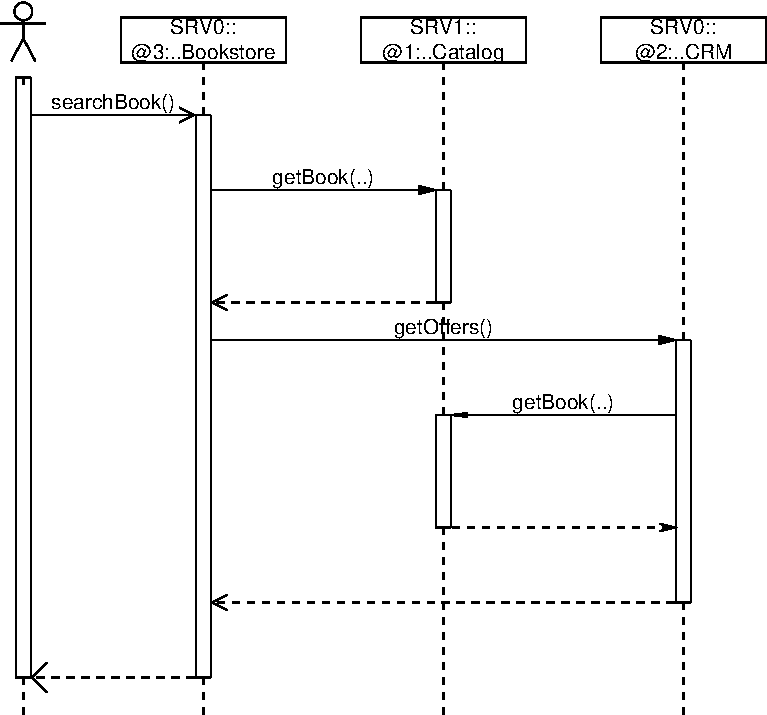
\includegraphics[scale=0.4]{images/example-plots/deploymentSequenceDiagram-6488138950668976129-crop}
}
\subfigure{%
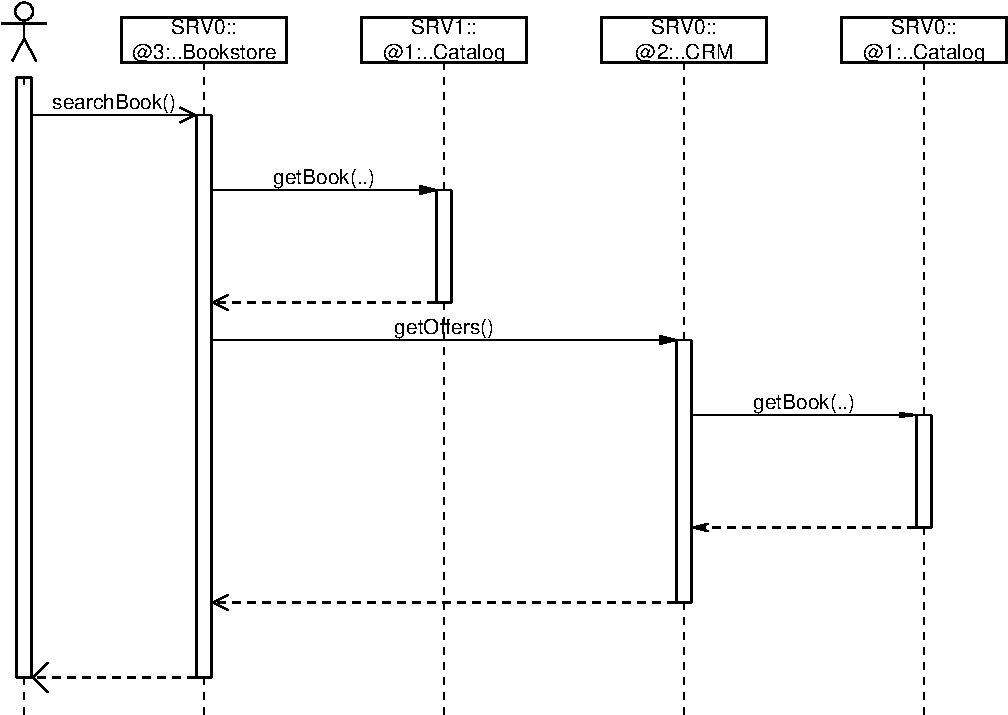
\includegraphics[scale=0.4]{images/example-plots/deploymentSequenceDiagram-6488138950668976130-crop}
}
\subfigure{%
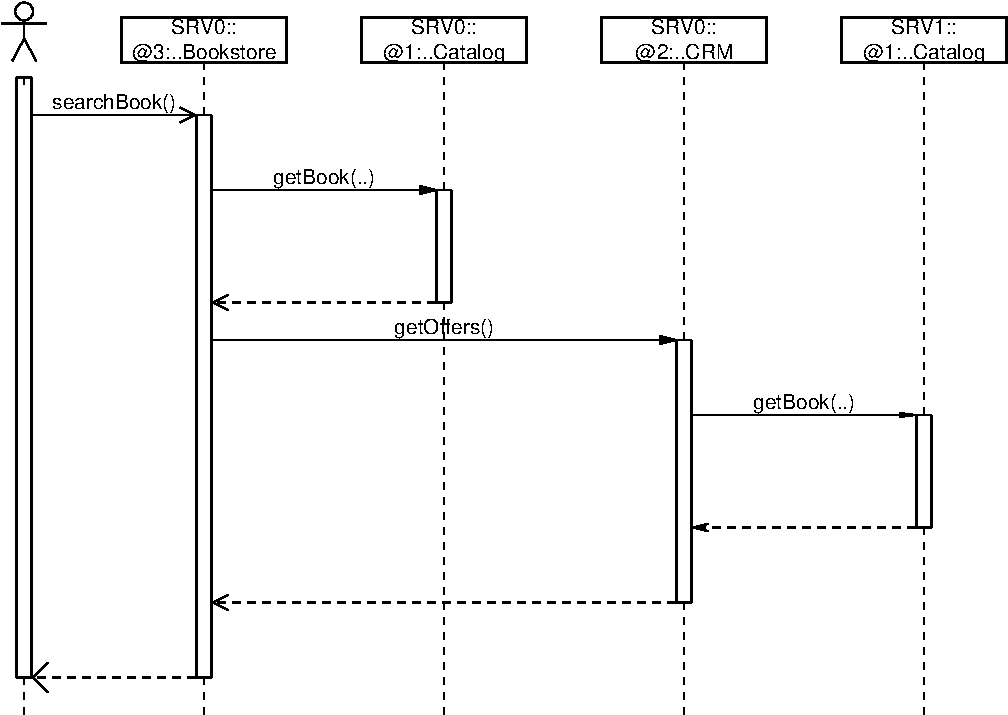
\includegraphics[scale=0.4]{images/example-plots/deploymentSequenceDiagram-6488138950668976131-crop}
}
\subfigure{%
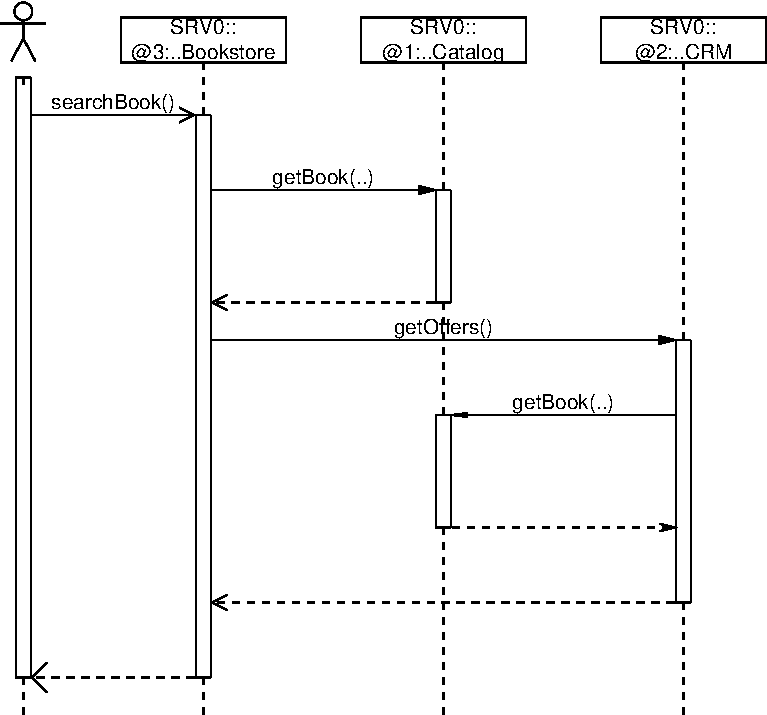
\includegraphics[scale=0.4]{images/example-plots/deploymentSequenceDiagram-6488138950668976141-crop}
}
\end{figure}

\newpage

\subsubsection{Assembly-Level Sequence Diagrams}

\begin{figure}[h]\centering
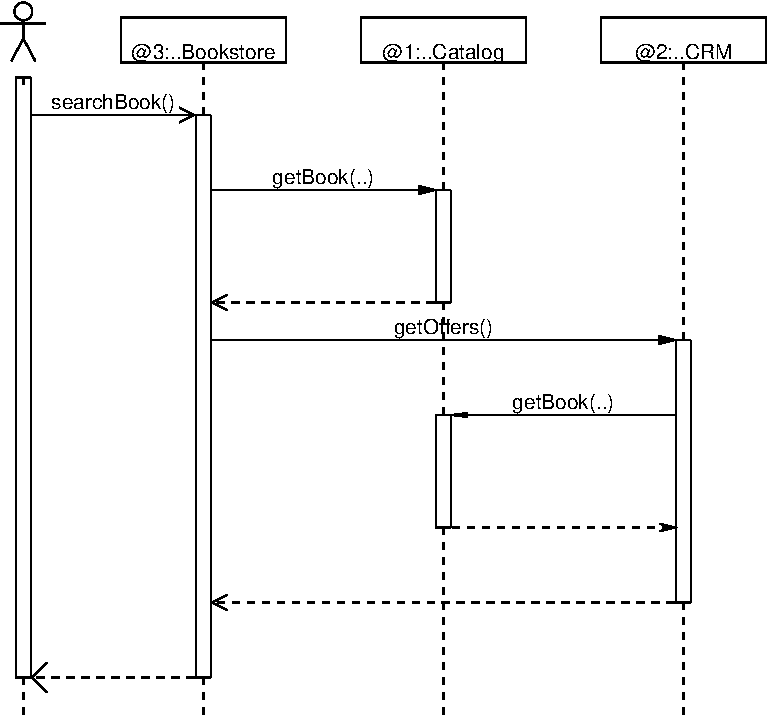
\includegraphics[scale=0.4]{images/example-plots/assemblySequenceDiagram-6488138950668976129-crop}
\end{figure}

\subsection{Call Trees}

\subsubsection{Trace Call Trees}

\begin{figure}[h]\centering
\subfigure{%
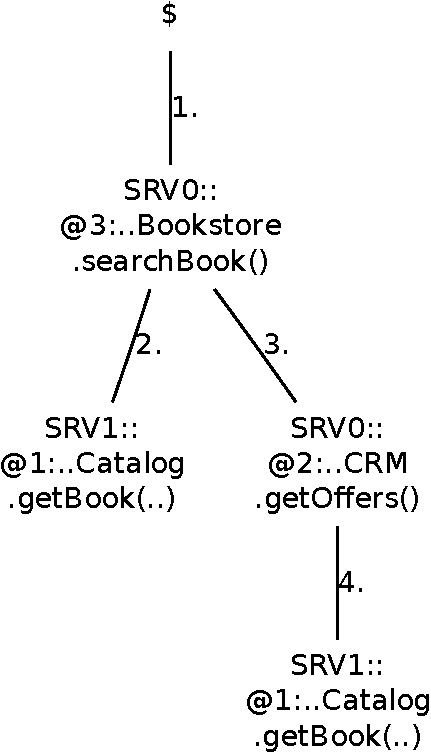
\includegraphics[scale=0.4]{images/example-plots/callTree-6488138950668976129-crop}
}
\subfigure{%
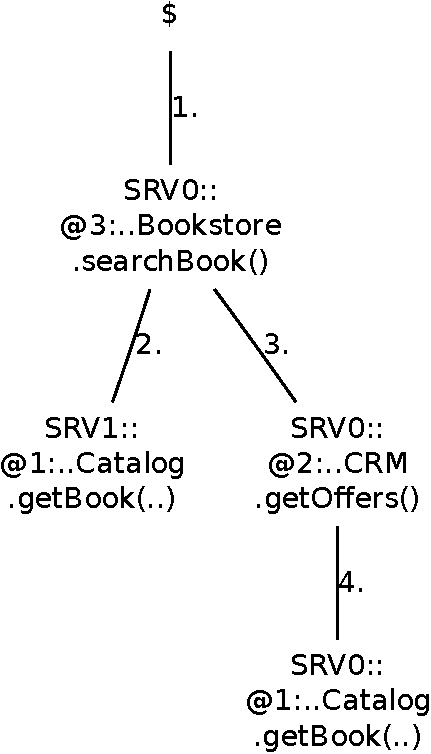
\includegraphics[scale=0.4]{images/example-plots/callTree-6488138950668976130-crop}
}
\subfigure{%
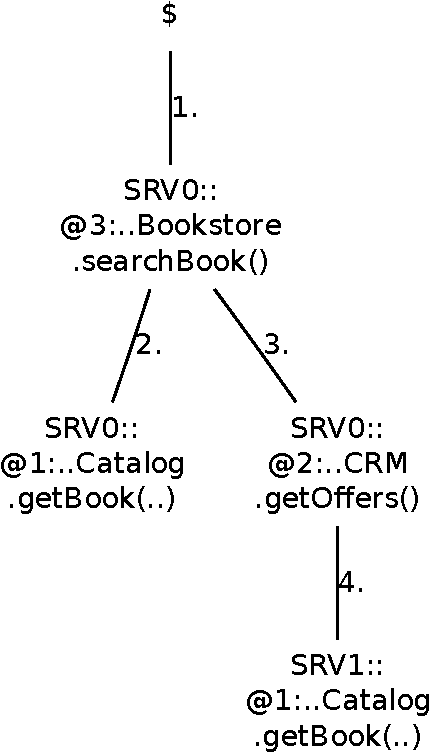
\includegraphics[scale=0.4]{images/example-plots/callTree-6488138950668976131-crop}
}
\subfigure{%
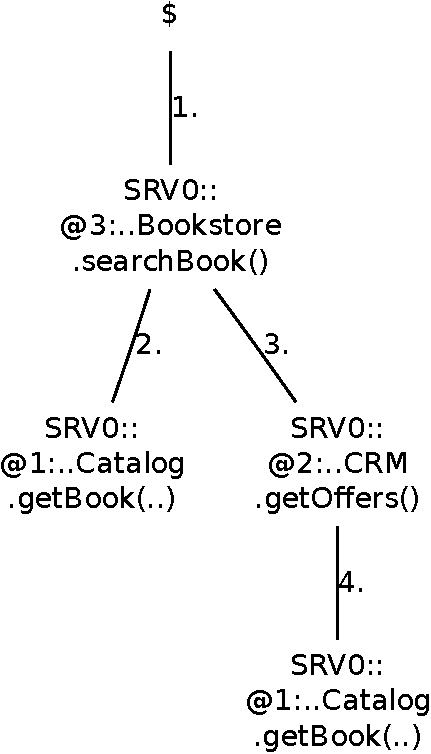
\includegraphics[scale=0.4]{images/example-plots/callTree-6488138950668976141-crop}
}
\end{figure}

\newpage

\subsubsection{Aggregated Call Trees}

\begin{figure}[h]\centering
\subfigure{%
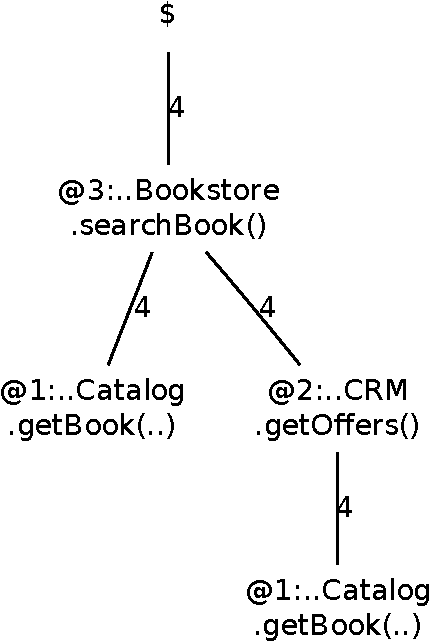
\includegraphics[scale=0.4]{images/example-plots/aggregatedAssemblyCallTree-crop}%
}
\subfigure{%
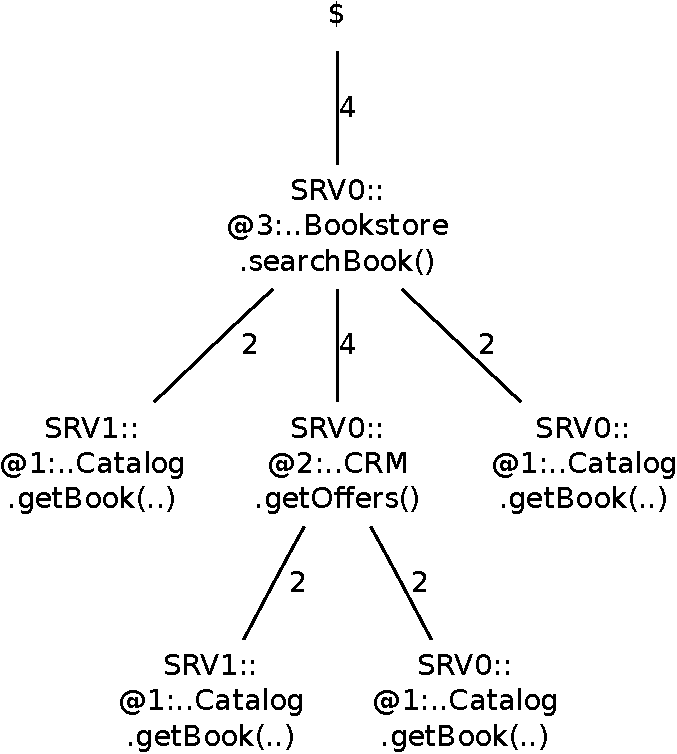
\includegraphics[scale=0.4]{images/example-plots/aggregatedDeploymentCallTree-crop}%
}
\end{figure}


\subsection{Dependency Graphs}

\subsubsection{Container Dependency Graphs}

\begin{figure}[h]\centering
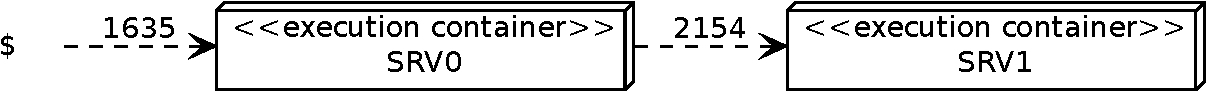
\includegraphics[scale=0.4]{images/example-plots/containerDependencyGraph-crop} 
\end{figure}

\subsubsection{Component Dependency Graphs}

\begin{figure}[h]\centering
\subfigure{%
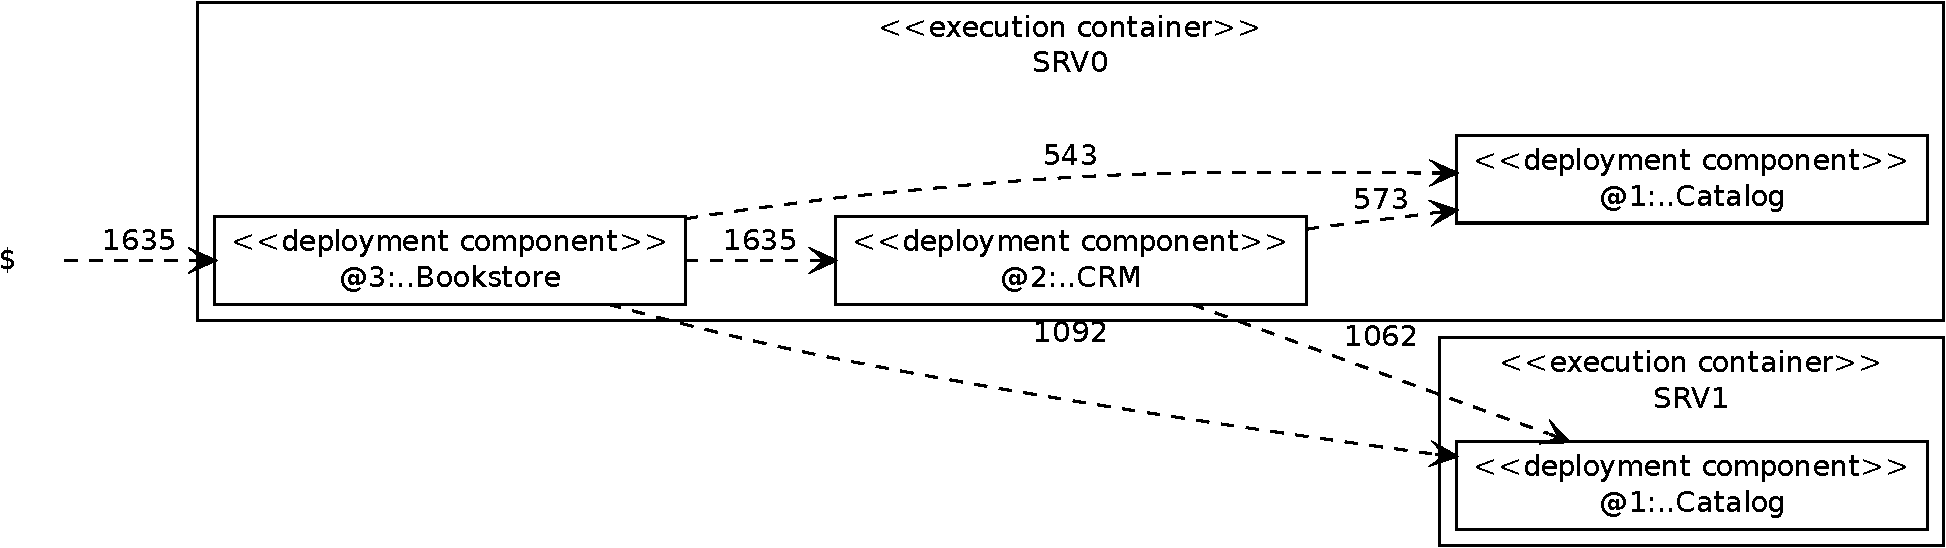
\includegraphics[scale=0.4]{images/example-plots/deploymentComponentDependencyGraph-crop}
}
\subfigure{%
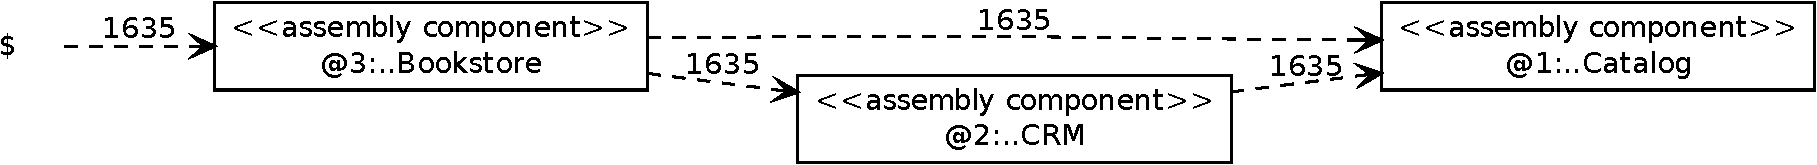
\includegraphics[scale=0.4]{images/example-plots/assemblyComponentDependencyGraph-crop}
}
\end{figure}


\subsubsection{Operation Dependency Graphs}



\enlargethispage{2cm}
	\begin{figure}[H]\centering
	\subfigure[deployment level]{\label{fig:appendix:allocationSequenceDiagram}
	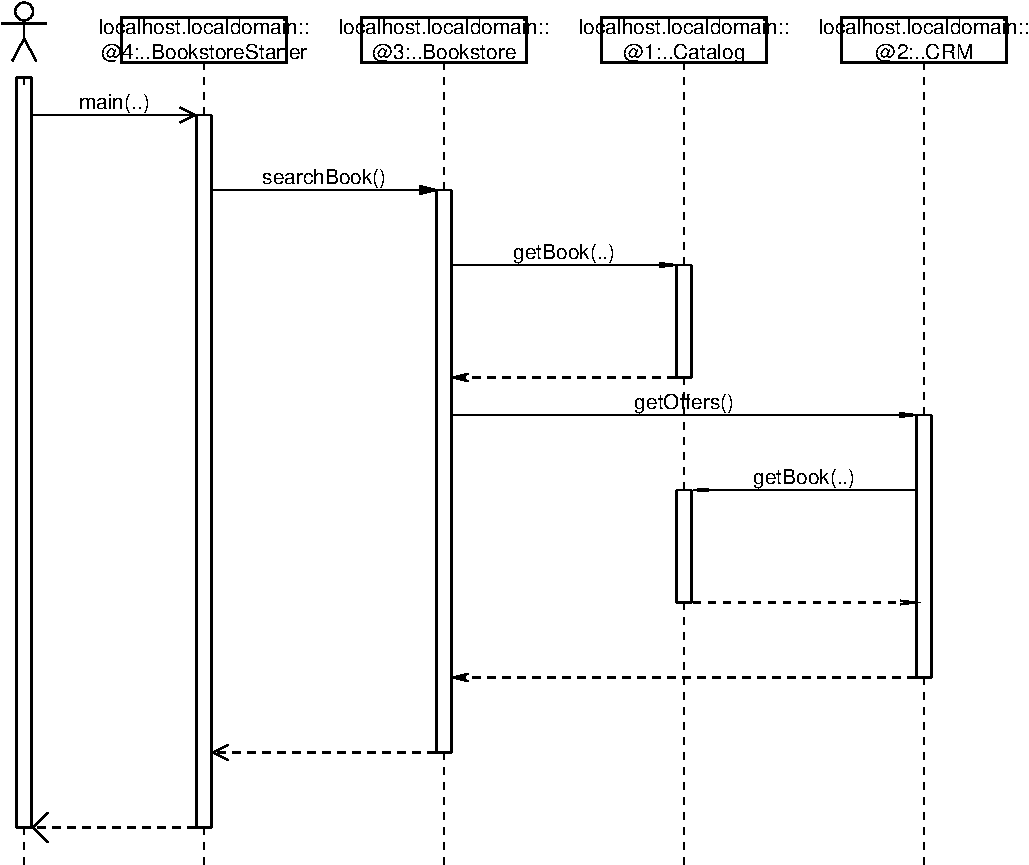
\includegraphics[scale=0.4]{images/allocationSequenceDiagram-crop}
	}
	\subfigure[assembly level]{\label{fig:appendix:assemblySequenceDiagram}
	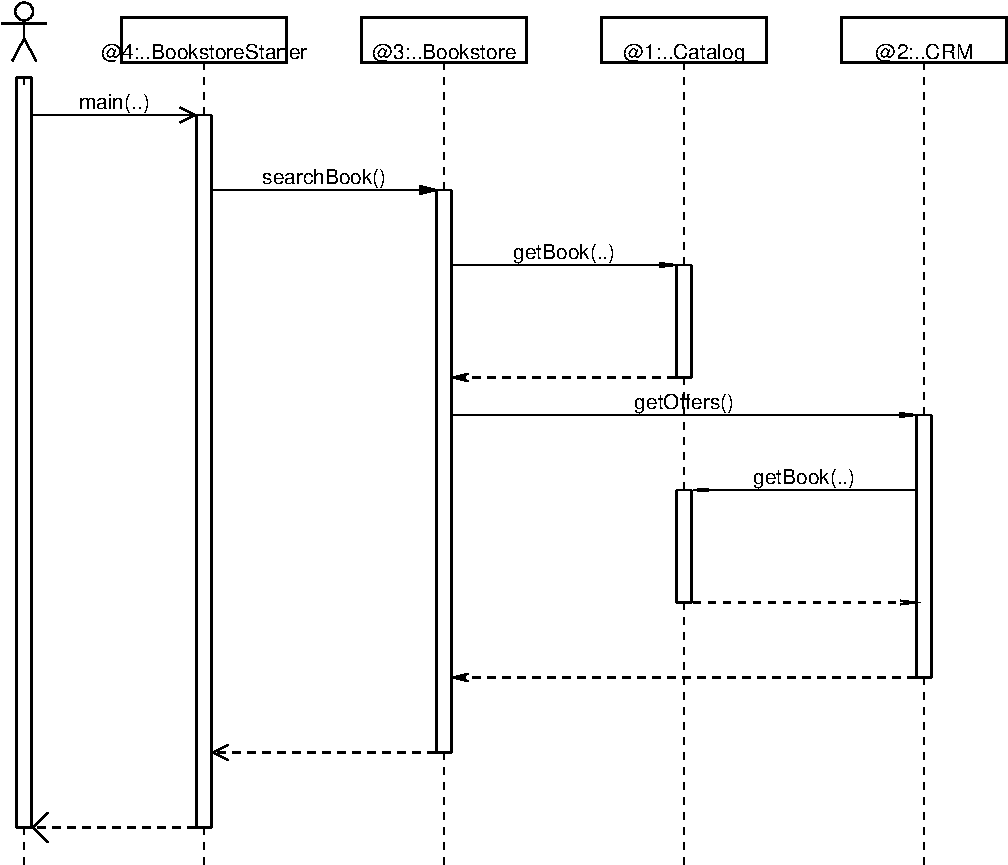
\includegraphics[scale=0.4]{images/assemblySequenceDiagram-crop}
	}
	\caption{Sequence diagrams}
	\end{figure}

    \begin{figure}[H]\centering
	\subfigure[single trace]{\label{fig:appendix:callTree}%
	\quad 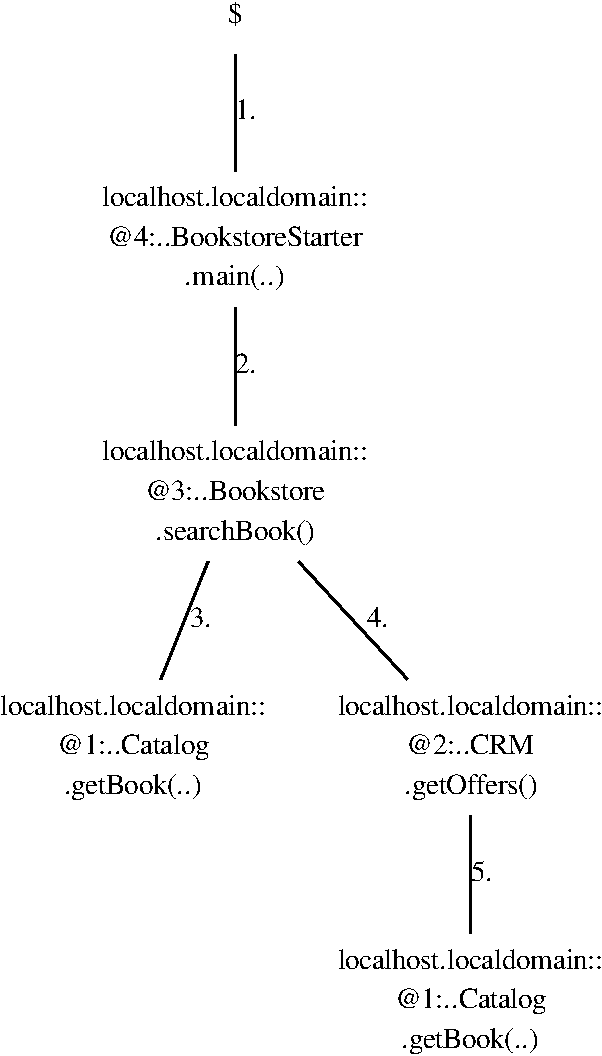
\includegraphics[scale=0.4]{images/callTree-crop} \quad%
	}%
	\subfigure[aggregated (deployment level)]{\label{fig:appendix:aggregatedAllocationCallTree}%
	\quad\quad 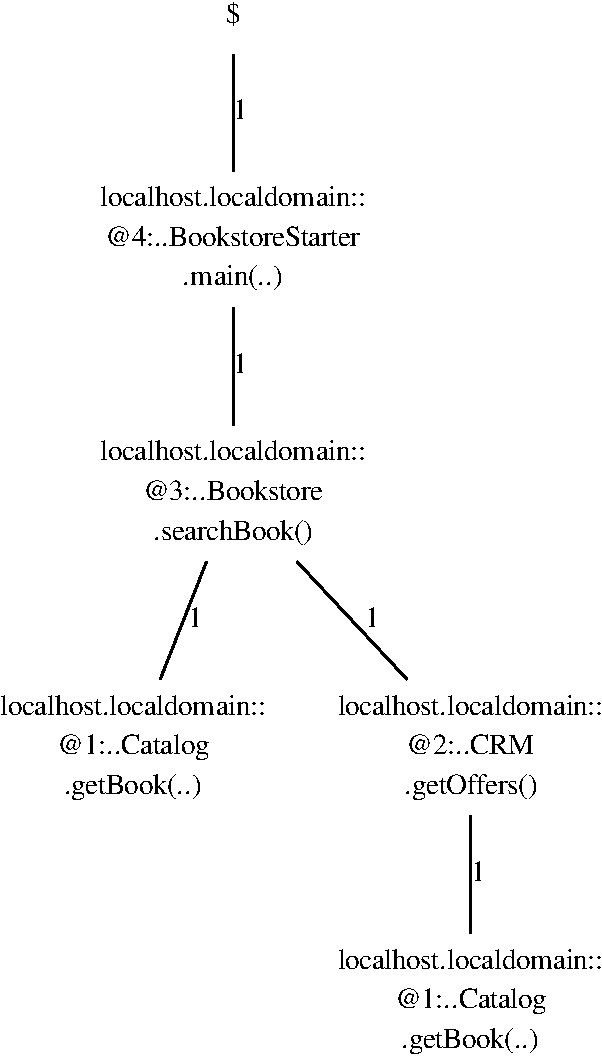
\includegraphics[scale=0.4]{images/aggregatedAllocationCallTree-crop}\quad\quad %
	}%
	\subfigure[aggregated (assembly level)]{\label{fig:appendix:aggregatedAssemblyCallTree}%
	\quad\quad\quad 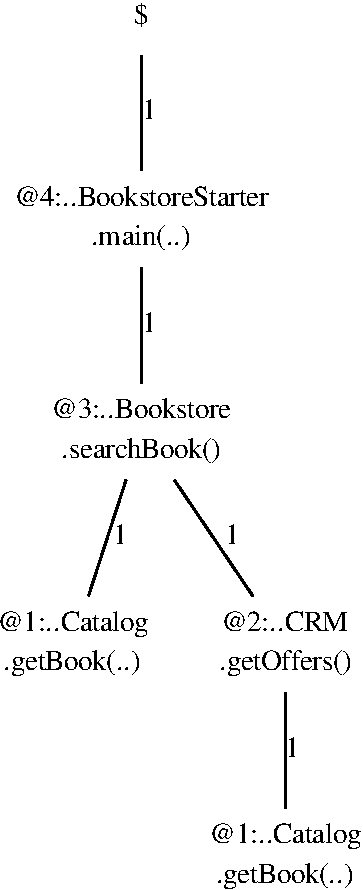
\includegraphics[scale=0.4]{images/aggregatedAssemblyCallTree-crop}\quad\quad\quad %
	}%
	\caption{Calls trees for a single trace~\subref{fig:appendix:callTree} and aggregated call %
	trees~\subref{fig:appendix:aggregatedAllocationCallTree}/\subref{fig:appendix:aggregatedAssemblyCallTree}}
	\end{figure}

\newpage

	\begin{figure}[H]
		\centering
		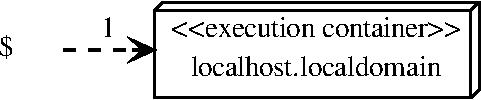
\includegraphics[scale=0.45]{images/containerDependencyGraph-crop}
		\caption{Container Dependency Graph}
	\end{figure}  

    \begin{figure}[H]\centering
\subfigure[deployment level]{\label{fig:appendix:allocationComponentDependencyGraph}%
		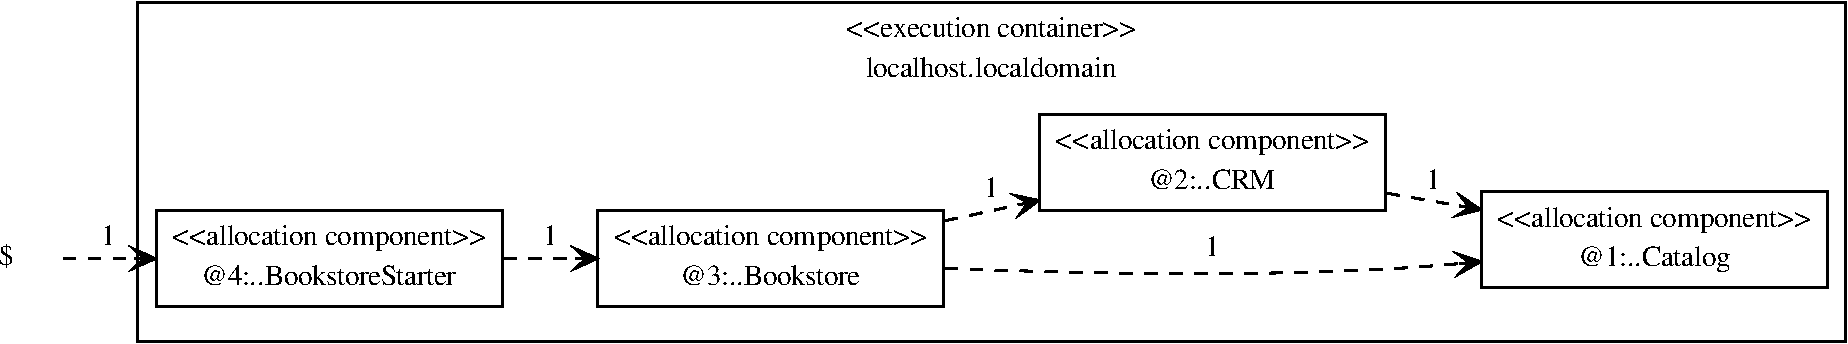
\includegraphics[scale=0.45]{images/allocationComponentDependencyGraph-crop}
	}\\
	\subfigure[assembly level]{\label{fig:appendix:assemblyComponentDependencyGraph}%
		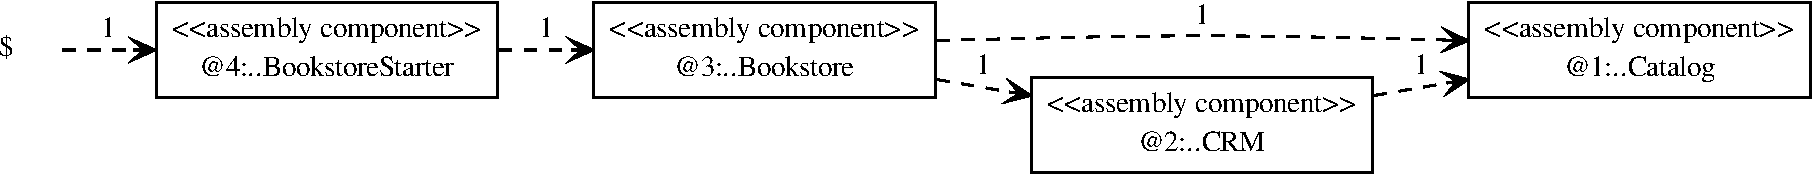
\includegraphics[scale=0.45]{images/assemblyComponentDependencyGraph-crop}
	}%
	\caption{Component Dependency Graphs}
	\end{figure}

	\begin{figure}[H]\centering
	\subfigure[deployment level]{\label{fig:appendix:allocationOperationDependencyGraph}%
		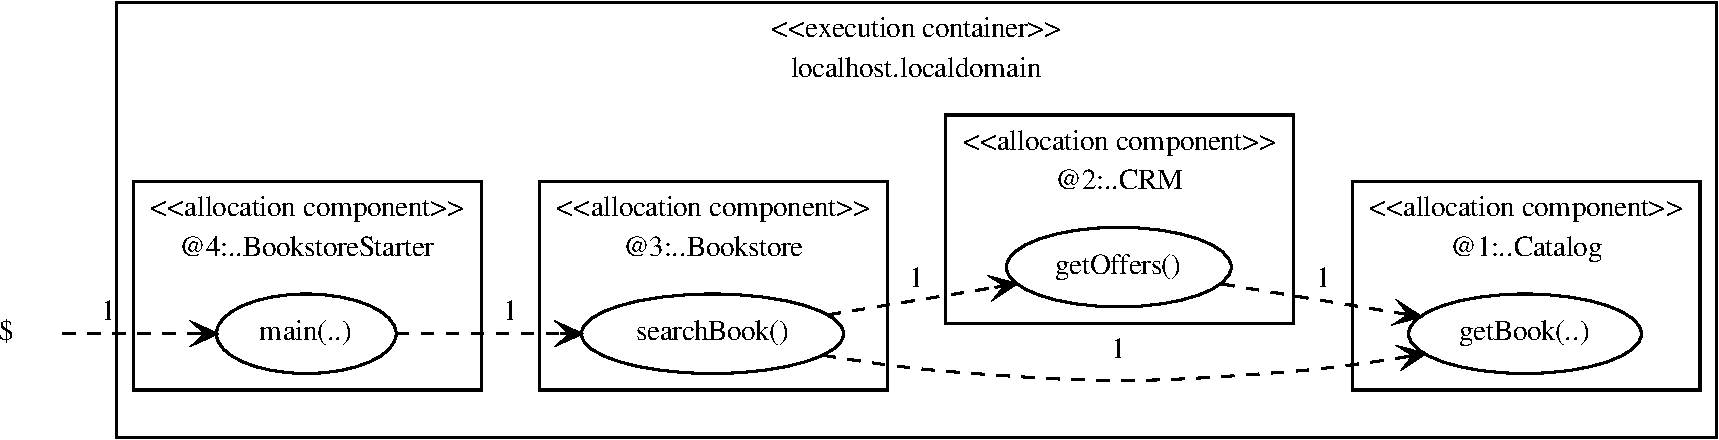
\includegraphics[scale=0.45]{images/allocationOperationDependencyGraph-crop}
	}\\
	\subfigure[assembly level]{\label{fig:appendix:assemblyOperationDependencyGraph}%
		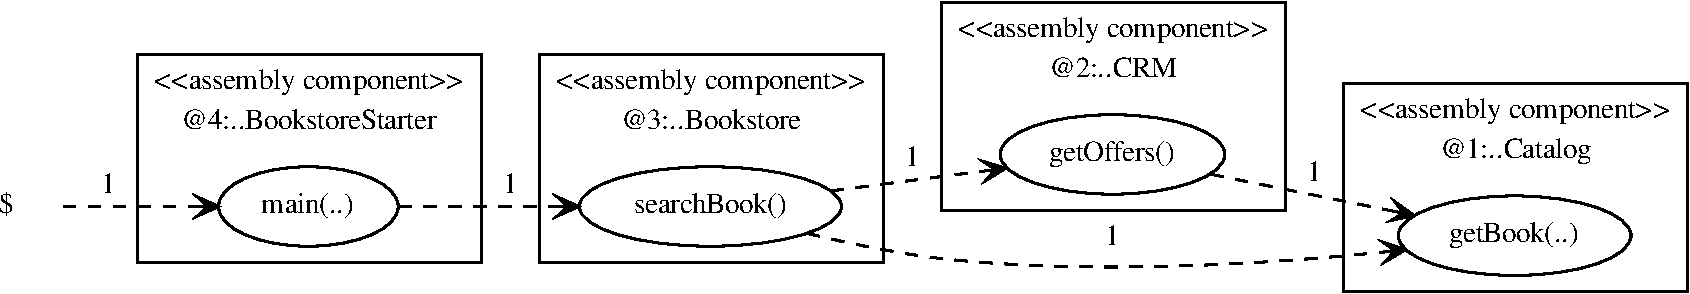
\includegraphics[scale=0.45]{images/assemblyOperationDependencyGraph-crop}
	}%
	\caption{Operation Dependency Graphs}
	\end{figure}

\chapter{Using the JMS Writer and Reader}\label{appendix:usingJMS}

This chapter gives a brief description on how to use the \class{AsyncJMSWriter} and \class{JMSReader} %
classes. This example is based on the Bookstore %
application with manual instrumentation presented in Chapter~\ref{chap:example}. %
The directory \dir{\JMSBookstoreApplicationDirDistro/} contains the %
sources, ant scripts etc. 

% \paragraph*{Preparation}

\begin{compactenum}
\item Copy the files \file{\mainJar} and \file{\commonsLoggingJar} from the %
binary distribution to the example's \dir{lib/} directory.
\item The file \file{\JMSBookstoreApplicationDirDistro/META-INF/kieker.monitoring.\-pro\-perties} %
is already configured to use the \class{AsyncJMSWriter}:
\end{compactenum}

\setPropertiesListing
\lstinputlisting[firstline=40,lastline=42,caption=Excerpt from \file{kieker.monitoring.properties} configuring the JMS writer]{\JMSBookstoreApplicationDir/META-INF/kieker.monitoring.properties}

\begin{compactenum}\setcounter{enumi}{2}
\item Download an OpenJMS install archive from \url{http://openjms.sourceforge.net} %
and decompress it to the root directory of the example. 
\item Copy the following files from the OpenJMS \dir{lib/} folder to the \dir{lib/} directory 
   of this example:
\begin{compactenum}
\item \file{openjms-<version>.jar}
\item \file{openjms-common-<version>.jar}
\item \file{openjms-net-<version>.jar}
\item \file{jms-<version>.jar}
\item \file{concurrent-<version>.jar}
\item \file{spice-jndikit-<version>.jar}
\end{compactenum}
\end{compactenum}

\enlargethispage{2cm}

% \paragraph*{Execution}%
 The execution of the example is performed by the following three steps:
\begin{enumerate}
\item Start the JMS server (you may have to set your \class{JAVA\_HOME} variable first):

\setBashListing
\begin{lstlisting}[caption=]
#\lstshellprompt{}# openjms-<version>/bin/startup.sh
\end{lstlisting}
\item Start the analysis part (in a new terminal):
\setBashListing
\begin{lstlisting}[caption=]
#\lstshellprompt{}# ant run-analysis
\end{lstlisting}
\item Start the instrumented Bookstore (in a new terminal):
\setBashListing
\begin{lstlisting}[caption=]
#\lstshellprompt{}# ant run-monitoring
\end{lstlisting}
\end{enumerate}

\chapter{Libraries}
    The following table shows all libraries which are used by \Kieker\ and explains them briefly.
    \begin{center}
\begin{longtable}{|p{0.4\textwidth}|p{0.5\textwidth}|}
\hline 
Filename & Description\\
\hline
\hline 
commons-cli-1.2.jar & n/a\\
\hline 
maven & n/a\\
\hline 
mysql-connector-java-5.1.5-bin.jar & The library to connect to an existing MySQL database.\\
\hline 
spring-web.jar & n/a\\
\hline 
Scenario.jar & n/a\\
\hline 
sequence.pic & n/a\\
\hline 
openjms-0.7.7-beta-1.tar.gz & n/a\\
\hline 
aspectjrt-1.6.6.jar & n/a\\
\hline 
commons-logging-1.1.1.jar & n/a\\
\hline 
aspectjtools-1.6.6.jar & n/a\\
\hline 
jms-1.1.jar & n/a\\
\hline 
concurrent-1.3.4.jar & n/a\\
\hline 
servlet.jar & n/a\\
\hline 
pmd & n/a\\
\hline 
spring.jar & n/a\\
\hline 
openjms-common-0.7.7-beta-1.jar & n/a\\
\hline 
servlet-api.jar & n/a\\
\hline 
commons-pool-1.2.jar & n/a\\
\hline 
derby.jar & This library contains the necessary drivers for the Apache Derby database.\\
\hline 
commons-io-1.2.jar & n/a\\
\hline 
cxf-rt-core-2.2.6.jar & n/a\\
\hline 
jmc.jar & n/a\\
\hline 
log4j-1.2.15.jar & n/a\\
\hline 
openjms-net-0.7.7-beta-1.jar & n/a\\
\hline 
aspectjweaver-1.6.6.jar & n/a\\
\hline 
cxf-api-2.2.6.jar & n/a\\
\hline 
rabbitmq-client.jar & n/a\\
\hline 
openjms-0.7.7-beta-1.jar & n/a\\
\hline 
spice-jndikit-1.2.jar & n/a\\
\hline 
cxf-rt-bindings-soap-2.2.6.jar & n/a\\
\hline 
cxf-common-utilities-2.2.6.jar & n/a\\
\hline 
jndi-1.2.1.jar & n/a\\
\hline 
\end{longtable}
\label{tabular:libraries}
\end{center}


% \chapter{Troubleshooting}
